\begin{figure}
\centering
    \begin{subfigure}{0.48\linewidth}
        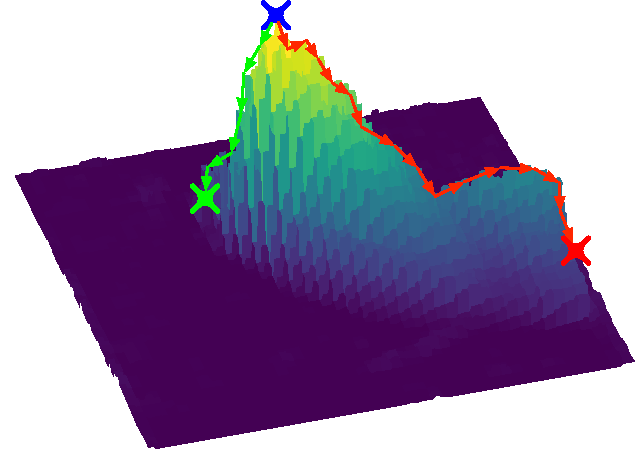
\includegraphics[width=\linewidth]{./img/scene_learning/ridge_climbing.pdf}
        \subcaption{}
        \label{subfig:scene-ridge-climbing}
    \end{subfigure}
    \begin{subfigure}{0.48\linewidth}
        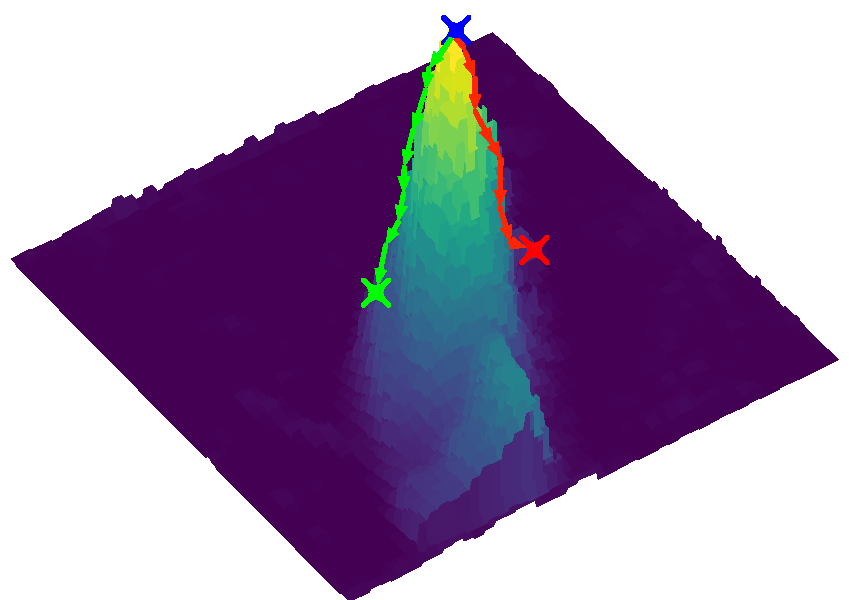
\includegraphics[width=\linewidth]{./img/scene_learning/ridge_climbing_perp.pdf}
        \subcaption{}
        \label{subfig:scene-ridge-climbing-perp}
    \end{subfigure}%
    \caption{3D visualization of the distribution of the first topic in \ref{fig:scene-topics} and ridge climbing illustration on it: along the dominant topic direction (\subref{subfig:scene-ridge-climbing}) and its perpendicular direction (\subref{subfig:scene-ridge-climbing-perp}). Blue cross indicates the starting point, red and green point indicates the end point.}
    \label{fig:scene-ridge-clibming}
\end{figure}